\documentclass[10pt, conference, compsocconf]{IEEEtran}
% Add the compsocconf option for Computer Society conferences.
%
% If IEEEtran.cls has not been installed into the LaTeX system files,
% manually specify the path to it like:
% \documentclass[conference]{../sty/IEEEtran}
\usepackage{cite}

\usepackage[cmex10]{amsmath}
\usepackage{amssymb}

\usepackage{algorithm}
\usepackage{array}
\usepackage{algpseudocode}
\usepackage{indentfirst}
\usepackage[pdftex]{graphicx}
\usepackage[tight,footnotesize]{subfigure}


%\usepackage{algorithmic}


\begin{document}

\title{Evaluation of Optimum Arithmetic Operators For Approximate Datapath Design}



\author{\IEEEauthorblockN{Kan Shi and George A. Constantinides}
\IEEEauthorblockA{Department of Electrical and Electronic Engineering\\
Imperial College London\\
London, UK\\
Email: {k.shi11, g.contantinides}@imperial.ac.uk}
%\and
%\IEEEauthorblockN{Authors Name/s per 2nd Affiliation (Author)}
%\IEEEauthorblockA{line 1 (of Affiliation): dept. name of organization\\
%line 2: name of organization, acronyms acceptable\\
%line 3: City, Country\\
%line 4: Email: name@xyz.com}
}


\maketitle


\begin{abstract}
The abstract goes here. 

\end{abstract}

\begin{IEEEkeywords}
approximate computing; datapath; computer arithmetic;

\end{IEEEkeywords}


\section{Introduction}

\section{Background}
\subsection{Approximate Datapath Design}

\subsection{Online Arithmetic}

Online arithmetic has been found using in numerous applications such as signal processing and control algorithms~\cite{Online_FPGADSP,Online_Control}. Online arithmetic was originally designed for digit-serial operation, as illustrated in Fig~\ref{Fig:OnlineDataFlow}. It can be seen that in order to generate the first output digit, $\delta$ digits of inputs are required, where $\delta$ is called the ``online delay''. $\delta$ is normally a small constant, which is independent of the precision. For ease of discussion, for the rest of this paper, the input data is assumed to be fixed point numbers in the range $(-1,1)$. Based on this premise, the online representation of $N$-digit operands and result at iteration $j$ are given by (\ref{Eq:Online_Operands}), where $j\in[-\delta,N-1]$ and $r$ denotes the radix \cite{Ercegovac_Book}.
%
\begin{figure}[tbp]
  \centering
  %\vspace{-2.5ex}
  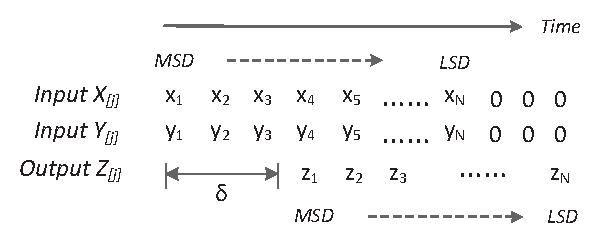
\includegraphics[width=.42\textwidth]{./figures/OnlineArithmetic_DataFlow.eps}
  %\vspace{-1ex}
  \caption{Dataflow in digit-serial online arithmetic, in which both inputs and outputs are processed from the MSD to the LSD. $\delta$ denotes the online delay.}
  \vspace{-2ex}
  \label{Fig:OnlineDataFlow}
\end{figure}
%
\begin{eqnarray}\label{Eq:Online_Operands}
\footnotesize
  X_{[j]}=\sum_{i=1}^{j+\delta}x_ir^{-i},~Y_{[j]}=\sum_{i=1}^{j+\delta}y_ir^{-i},~Z_{[j]}=\sum_{i=1}^{j}z_ir^{-i}
\normalsize
\end{eqnarray}

MSD-first operation is possible only if a redundant number system is used. Normally there are two most commonly used redundant number representations: carry-save (CS) \cite{CSadder} and signed-digit (SD) \cite{RedundantNumber}. With SD representation, each digit is represented using a redundant digit set $\{-a, \cdots,-1,0, 1, \cdots, a\}$, where $a\in[r/2,r-1]$. In comparison, the standard non-redundant representation only uses a digit set $\{0,\cdots,r-1\}$. Thus a standard number corresponds to several possible redundant representations. For example, the binary number $0.011$ can be represented in SD form as $0.1\overline{1}1$, $0.10\overline{1}$ or $0.011$ among many other possible representations.

Due to the redundancy, the MSDs of the result can be calculated using partial information from both inputs. Then the value of the number can be revised using the subsequent digits, because each number has multiple representations.

\section{Comparison of Different Adder Structures}
\subsection{Ripple Carry Adder}
Adders serve as a key building block for arithmetic operations. In general, the ripple carry adder (RCA) is the most straightforward and widely used adder structure. As such, in our previous work we proposed probabilistic models of overclocking errors for RCA.

For an $n$-bit RCA, it is composed of $n$ serial-connected full adders (FA). Typically the maximum frequency of RCA is determined by the longest carry propagation. Under the assumption that the carry propagation delay of each FA is a constant value $\mu$, the critical path of the RCA is: $\mu_{RCA}=n\mu$. For the sampling period $T_S$, it follows that if $T_S\geqslant\mu_{RCA}$, correct result will always be sampled; otherwise if $T_S<\mu_{RCA}$, intermediate be sampled and potentially generating errors. In the previous work, the mean value of overclocking error is modeled as given in (\ref{Eq:MeanError_RCA}), where coefficient $b$ is given in (\ref{Eq:b}) and it determines the maximum length of error-free carry propagation in bits.
%
\begin{eqnarray}\label{Eq:MeanError_RCA}
    E_O=\left\{
        \begin{matrix}
            2^{-b}-2^{-n-1}, & \textrm{if $b\leq n$}\\
            0, & \textrm{otherwise}
        \end{matrix}
        \right.
\end{eqnarray}
%
\begin{eqnarray}\label{Eq:b}
    b:=\left\lceil \frac{T_S}{\mu} \right\rceil=\left\lceil \frac{1}{\mu\cdot f_S}\right\rceil
\end{eqnarray}

On the other hand, a specific timing target can be met by truncating the word-length of RCA while timing violation is not permitted. This will result in truncation error for most data.  The mean value of truncation error is also modeled as given in~(\ref{Eq:MeanTruncError_RCA}) [xxx], where parameters $k$ and $n$ denote the word-length of RCA before and after truncation, respectively. 
%
\begin{eqnarray}\label{Eq:MeanTruncError_RCA}
    E_O=\left\{
        \begin{matrix}
            2^{-n}-2^{-k}, & \textrm{if $n<k$}\\
            0, & \textrm{otherwise}
        \end{matrix}
        \right.
\end{eqnarray}

In this paper we consider two design scenarios for RCA: one is the overclocking scenario where timing violation is allowed to happen while maintaining the original word-length; the other is the trad scenario by truncating RCA word-length to meet timing. For a given $f_S$, in the first design scenario we have $n=k$. In the second design scenario we have $n=b-1$ to prevent timing violation while minimizing the value of $E_O$. Therefore the comparison between the two scenarios in mean error value is given in (\ref{Eq:ErrorCompare_RCA}) by updating (\ref{Eq:MeanError_RCA}) and (\ref{Eq:MeanTruncError_RCA}) respectively. As seen in (\ref{Eq:ErrorCompare_RCA}), in theory the mean value of error in the overclocking scenario ($E_{oc}$) is two times smaller than that in the traditional scenario ($E_{trad}$).
%
\begin{eqnarray}\label{Eq:ErrorCompare_RCA}
    \frac{E_{oc}}{E_{trad}} = \frac{2^{-b}-2^{-n-1}|_{n=k}}{2^{-n}-2^{-k}|_{n=b-1}}=\frac{1}{2}
\end{eqnarray}

\subsection{Carry Select Adder}



\subsection{Online Adder}
\subsubsection{Algorithm}
The structure of a digit-parallel online adder where all signals represented with SD numbers of digit set $\{-1,0,1\}$ is shown in Fig.~\ref{Fig:Radix2SD_adder}. The module ``3:2'' denotes a 3:2 compressor, which takes three inputs and generates two outputs, and is logically equivalent to a full adder (FA). A major advantage of the redundant number system over the standard ripple-carry based arithmetic is that the propagation of carry is eliminated, resulting in a precision-independent computation time for addition. As labelled in Fig.~\ref{Fig:Radix2SD_adder}, ideally the computation delay of this adder is only two FA delays for any operand word-length, with the cost of one extra FA for each digit of operands. This makes the online adder suitable for building up more complex arithmetic operators such as multipliers to accelerate the sum of partial products \cite{RedundantMult_1987}.
%
\begin{figure}[tbp]
  \centering
  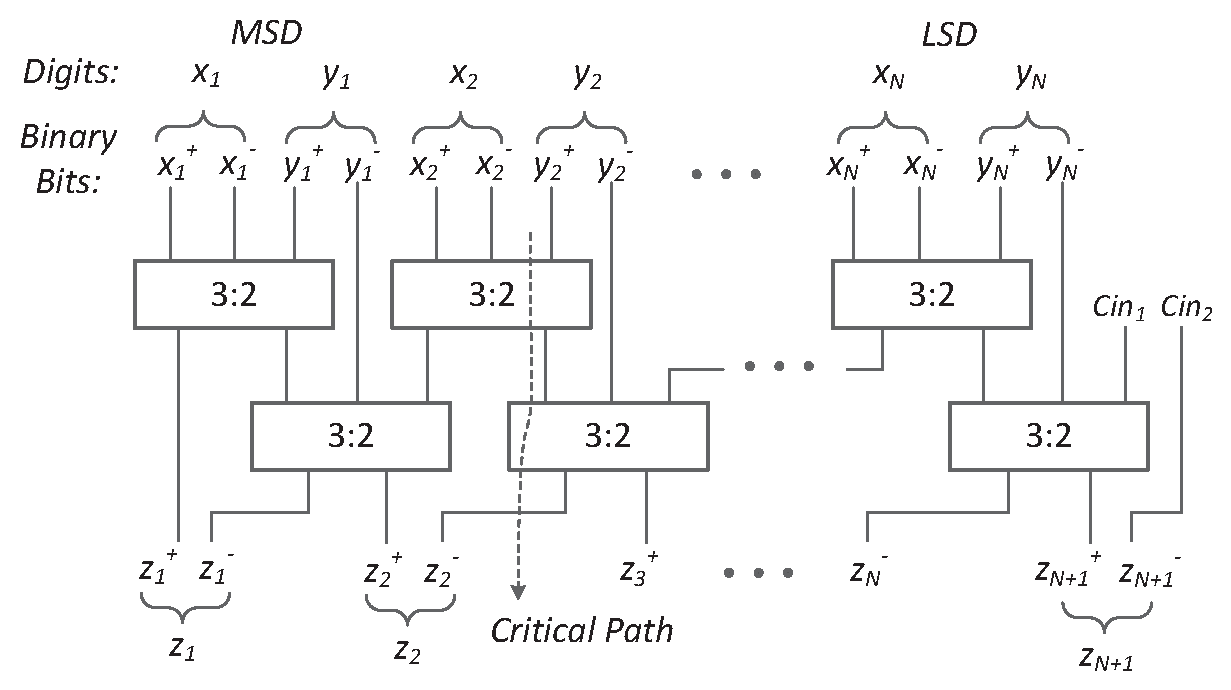
\includegraphics[width=.45\textwidth]{./figures/SDAdder.eps}
  %\vspace{-7ex}
  %\vspace{-2ex}
  \caption{An $N$-digit binary digit-parallel online adder. Both inputs and outputs are represented using SD representation. ``3:2'' denotes a 3:2 compressor.}
    \vspace{-2ex}
  \label{Fig:Radix2SD_adder}
\end{figure}

\begin{eqnarray}\label{Eq:b}
    b:=\left\lceil \frac{T_S}{\mu} \right\rceil=\left\lceil \frac{1}{\mu\cdot f_S}\right\rceil
\end{eqnarray}



\section{Comparison of Different Multiplier Structures}
\subsection{Standard Binary Multiplier}

\subsection{Online Multiplier}
\subsubsection{Algorithm}
Similar to online addition, online multiplication can also be implemented in a unrolled digit-parallel manner, of which the optimized algorithm is shown in Algorithm~\ref{Algorithm:OM_DigitParallel} [xxx]. In this algorithm, both inputs and outputs are $N$-digit numbers as given in (\ref{Eq:Online_Operands}). For a given iteration $j$, the product digit $z_j$ is generated MSD-first through a selection function $sel()$. For any radix $r$ and chosen digit set, there exits an appropriate selection method and a value of $\delta$ which ensure convergence. As the binary radix is used most commonly in computer arithmetic, we keep $r=2$ throughout this paper with the corresponding redundant digit set $\{\overline{1},0,1\}$. In this case $sel()$ is given by (\ref{Eq:SelFunc_OM})~\cite{Ercegovac_OnlineMult}.

\begin{algorithm}[tbp]
  \caption{Digit Parallel Online Multiplication}\label{Algorithm:OM_DigitParallel}
  \begin{algorithmic}[1]
    \State \textbf{Initialization:} $P_{[0]}=0$                     \vspace{.5ex}
    \For{$j=1,~2,~\cdots,~N$}                                       \vspace{.5ex}
        \State $Xy_j \leftarrow X \cdot y_j$                        \vspace{.5ex}
        \State $W_{[j]}    \leftarrow  P_{[j-1]} + Xy_j$            \vspace{.5ex}
        \State $z_{j}  ~~      \leftarrow  sel(W_{[j]})$            \vspace{.5ex}
        \State $P_{[j+1]}  \leftarrow  r\left(W_{[j]}-Z_{[j]}\right)$   \vspace{.5ex}
    \EndFor                                                         \vspace{.5ex}
    \State $Z_{[N+1:2N]} \leftarrow frac(W_{[N]})$                  \vspace{.5ex}
  \end{algorithmic}
  \vspace{-1ex}
\end{algorithm}

\begin{eqnarray}\label{Eq:SelFunc_OM}
\small
  sel(W_{[j]})=\begin{cases}
    1 & \text{ if } W_{[j]} \geqslant \frac{1}{2} \\
    0 & \text{ if } -\frac{1}{2}\leqslant W_{[j]}<\frac{1}{2} \\
    \overline{1} & \text{ if } W_{[j]}<-\frac{1}{2}
  \end{cases}
\normalsize
\end{eqnarray}

In our previous work, an area efficient implementation 

\begin{figure}[tbp]
  \centering
  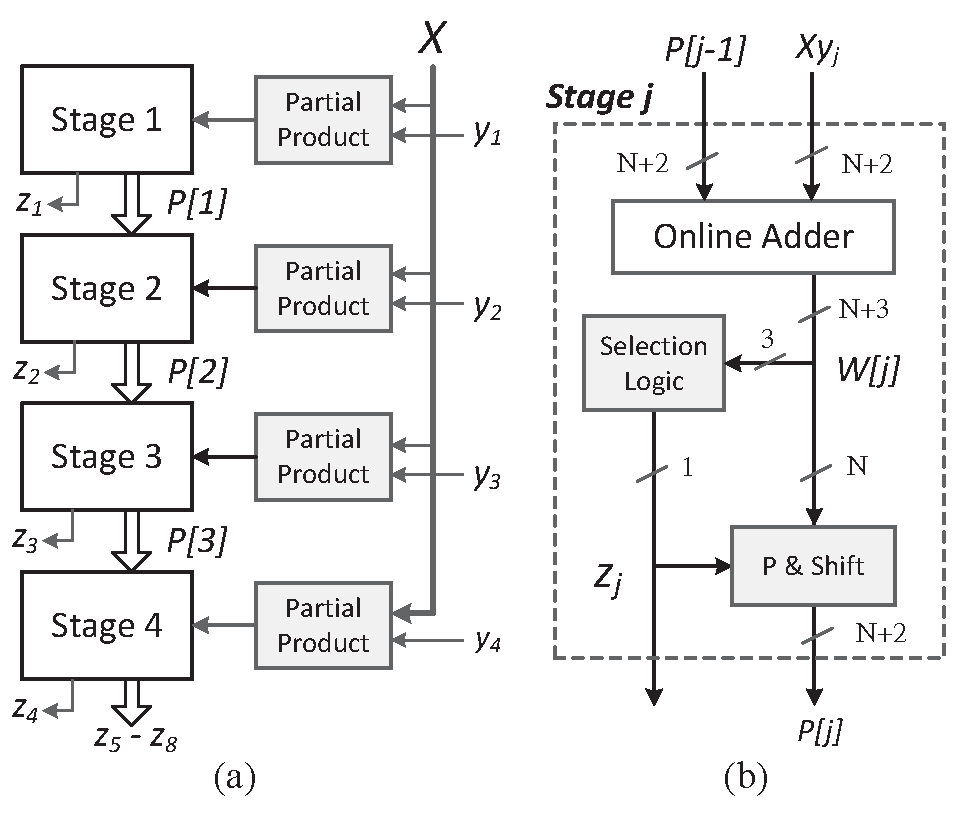
\includegraphics[width=.42\textwidth]{./figures/ParallelMult_Structure.eps}
  \caption{(a) Structure of a 4-digit online multiplier. (b) Structure of one stage. The word-length of all signals are labeled in digits, $N$ is the word-length of input signals.}
    \vspace{-2ex}
  \label{Fig:PM}
\end{figure}

\subsubsection{Structure Optimization for Half Precision Results}
In actual applications, normally the multiplier is connected with other arithmetic operators. If the multiplication result is utilized for subsequent operations, and a consistent word-length is used throughout the system, then only the most significant half of the product is required. In a conventional multiplier with standard binary arithmetic, this is achieved by either truncating or rounding the least significant half of the products. However, both the computation time and the structure remains unchanged, because results are generated from LSDs.

In comparison, OM offers the flexibility to simplify the structure corresponding to the required precision. This is possible because in an OM, the product digits are generated initially from the MSD, and there is no carry propagation from the LSD to the MSD with the employment of the redundant number system. This will potentially lead to a more area efficient design. For example, the modified structure diagram of a 4-digit OM is illustrated in Fig.~\ref{Fig:PM_half}(a). The word-length of signals within each stage can be correspondingly reduced, as shown in Fig.~\ref{Fig:PM_half}(b). Notice that instead of keeping identical word-length throughout the stages (in Fig.~\ref{Fig:PM}), in the modified structure the signal word-lengths depend on the stage number $j$ and hence fewer bits of signals are needed for LSD stages.

\begin{figure}[tbp]
  \centering
  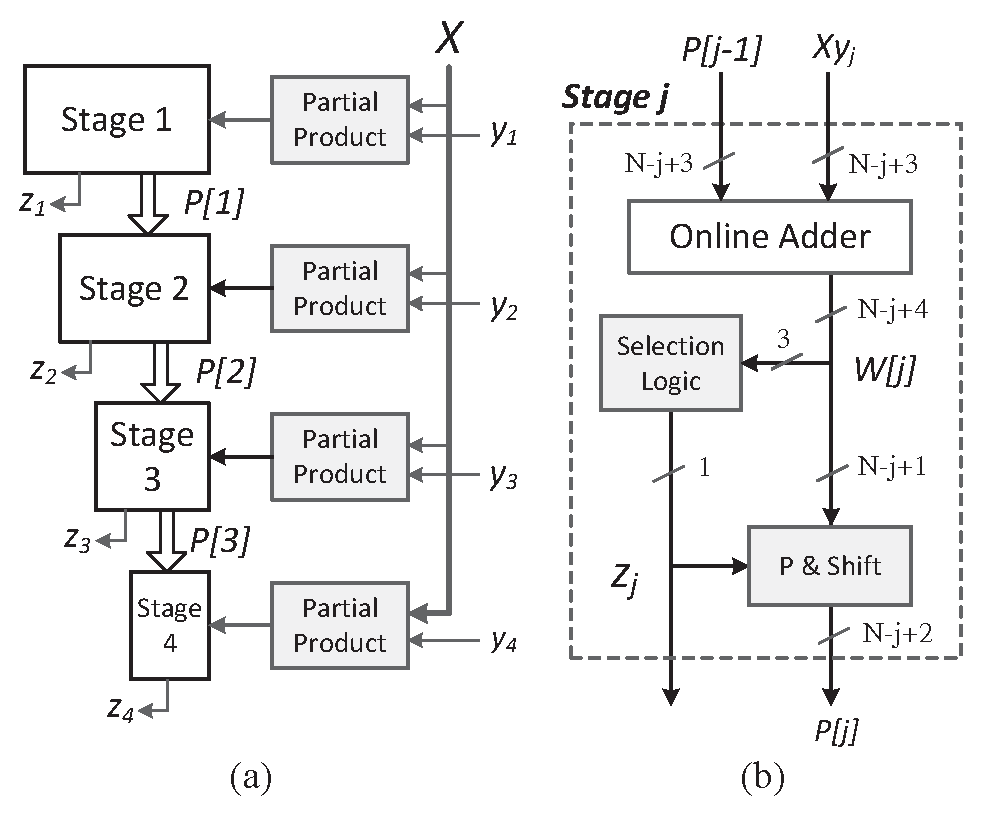
\includegraphics[width=.42\textwidth]{./figures/ParallelMult_MSDhalf.eps}
  \caption{(a) A 4-digit online multiplier with half precision results. (b) Structure of stage $j$, with the word-length of all signals labeled.}
    \vspace{-2ex}
  \label{Fig:PM_half}
\end{figure}

\section{Conclusion}

\section*{Acknowledgment}


\bibliographystyle{./IEEEtran}

\bibliography{./IEEEabrv,./Reference}


\end{document}


